% DRAFT v0 (2026-10-17). Every number comes from numbers.tex (generated by analysis/paper_numbers.py).
% Related work drafted from the systematic search (2026-10-18); citation keys are record ids in docs/lit-review/records.csv.
\documentclass[10pt]{article}
\usepackage[margin=2.2cm]{geometry}
\usepackage{graphicx,booktabs,hyperref,amsmath,pifont,microtype}
% GENERATED by analysis/paper_numbers.py from analysis/out/*.json - do not edit by hand.
\newcommand{\WzeroChains}{720}
\newcommand{\WzeroOverallSafeK}{680}
\newcommand{\WzeroOverallSafeN}{720}
\newcommand{\WzeroOverallSafePct}{94.4}
\newcommand{\WzeroOverallSafeLo}{92.5}
\newcommand{\WzeroOverallSafeHi}{95.9}
\newcommand{\WzeroOverallScannerCleanK}{714}
\newcommand{\WzeroOverallScannerCleanN}{720}
\newcommand{\WzeroOverallScannerCleanPct}{99.2}
\newcommand{\WzeroOverallScannerCleanLo}{98.2}
\newcommand{\WzeroOverallScannerCleanHi}{99.6}
\newcommand{\WzeroOverallRqoneBreakingAmongCleanK}{29}
\newcommand{\WzeroOverallRqoneBreakingAmongCleanN}{714}
\newcommand{\WzeroOverallRqoneBreakingAmongCleanPct}{4.1}
\newcommand{\WzeroOverallRqoneBreakingAmongCleanLo}{2.8}
\newcommand{\WzeroOverallRqoneBreakingAmongCleanHi}{5.8}
\newcommand{\WzeroOverallRqtwoDeceptiveAmongCleanK}{8}
\newcommand{\WzeroOverallRqtwoDeceptiveAmongCleanN}{714}
\newcommand{\WzeroOverallRqtwoDeceptiveAmongCleanPct}{1.1}
\newcommand{\WzeroOverallRqtwoDeceptiveAmongCleanLo}{0.6}
\newcommand{\WzeroOverallRqtwoDeceptiveAmongCleanHi}{2.2}
\newcommand{\WzeroCzeroViewScannerCleanK}{178}
\newcommand{\WzeroCzeroViewScannerCleanN}{180}
\newcommand{\WzeroCzeroViewScannerCleanPct}{98.9}
\newcommand{\WzeroCzeroViewScannerCleanLo}{96.0}
\newcommand{\WzeroCzeroViewScannerCleanHi}{99.7}
\newcommand{\WzeroCzeroViewOfWhichSafeK}{164}
\newcommand{\WzeroCzeroViewOfWhichSafeN}{178}
\newcommand{\WzeroCzeroViewOfWhichSafePct}{92.1}
\newcommand{\WzeroCzeroViewOfWhichSafeLo}{87.2}
\newcommand{\WzeroCzeroViewOfWhichSafeHi}{95.3}
\newcommand{\WzeroCzeroViewOfWhichBreakingK}{12}
\newcommand{\WzeroCzeroViewOfWhichBreakingN}{178}
\newcommand{\WzeroCzeroViewOfWhichBreakingPct}{6.7}
\newcommand{\WzeroCzeroViewOfWhichBreakingLo}{3.9}
\newcommand{\WzeroCzeroViewOfWhichBreakingHi}{11.4}
\newcommand{\WzeroCzeroViewOfWhichDeceptiveK}{2}
\newcommand{\WzeroCzeroViewOfWhichDeceptiveN}{178}
\newcommand{\WzeroCzeroViewOfWhichDeceptivePct}{1.1}
\newcommand{\WzeroCzeroViewOfWhichDeceptiveLo}{0.3}
\newcommand{\WzeroCzeroViewOfWhichDeceptiveHi}{4.0}
\newcommand{\WzeroDeepseekVthreetwoSafeK}{210}
\newcommand{\WzeroDeepseekVthreetwoSafeN}{240}
\newcommand{\WzeroDeepseekVthreetwoSafePct}{87.5}
\newcommand{\WzeroDeepseekVthreetwoSafeLo}{82.7}
\newcommand{\WzeroDeepseekVthreetwoSafeHi}{91.1}
\newcommand{\WzeroDeepseekVthreetwoScannerCleanK}{237}
\newcommand{\WzeroDeepseekVthreetwoScannerCleanN}{240}
\newcommand{\WzeroDeepseekVthreetwoScannerCleanPct}{98.8}
\newcommand{\WzeroDeepseekVthreetwoScannerCleanLo}{96.4}
\newcommand{\WzeroDeepseekVthreetwoScannerCleanHi}{99.6}
\newcommand{\WzeroDeepseekVthreetwoRqoneBreakingAmongCleanK}{27}
\newcommand{\WzeroDeepseekVthreetwoRqoneBreakingAmongCleanN}{237}
\newcommand{\WzeroDeepseekVthreetwoRqoneBreakingAmongCleanPct}{11.4}
\newcommand{\WzeroDeepseekVthreetwoRqoneBreakingAmongCleanLo}{7.9}
\newcommand{\WzeroDeepseekVthreetwoRqoneBreakingAmongCleanHi}{16.1}
\newcommand{\WzeroDeepseekVthreetwoRqtwoDeceptiveAmongCleanK}{3}
\newcommand{\WzeroDeepseekVthreetwoRqtwoDeceptiveAmongCleanN}{237}
\newcommand{\WzeroDeepseekVthreetwoRqtwoDeceptiveAmongCleanPct}{1.3}
\newcommand{\WzeroDeepseekVthreetwoRqtwoDeceptiveAmongCleanLo}{0.4}
\newcommand{\WzeroDeepseekVthreetwoRqtwoDeceptiveAmongCleanHi}{3.7}
\newcommand{\WzeroGlmfiveSafeK}{233}
\newcommand{\WzeroGlmfiveSafeN}{240}
\newcommand{\WzeroGlmfiveSafePct}{97.1}
\newcommand{\WzeroGlmfiveSafeLo}{94.1}
\newcommand{\WzeroGlmfiveSafeHi}{98.6}
\newcommand{\WzeroGlmfiveScannerCleanK}{240}
\newcommand{\WzeroGlmfiveScannerCleanN}{240}
\newcommand{\WzeroGlmfiveScannerCleanPct}{100.0}
\newcommand{\WzeroGlmfiveScannerCleanLo}{98.4}
\newcommand{\WzeroGlmfiveScannerCleanHi}{100.0}
\newcommand{\WzeroGlmfiveRqoneBreakingAmongCleanK}{2}
\newcommand{\WzeroGlmfiveRqoneBreakingAmongCleanN}{240}
\newcommand{\WzeroGlmfiveRqoneBreakingAmongCleanPct}{0.8}
\newcommand{\WzeroGlmfiveRqoneBreakingAmongCleanLo}{0.2}
\newcommand{\WzeroGlmfiveRqoneBreakingAmongCleanHi}{3.0}
\newcommand{\WzeroGlmfiveRqtwoDeceptiveAmongCleanK}{5}
\newcommand{\WzeroGlmfiveRqtwoDeceptiveAmongCleanN}{240}
\newcommand{\WzeroGlmfiveRqtwoDeceptiveAmongCleanPct}{2.1}
\newcommand{\WzeroGlmfiveRqtwoDeceptiveAmongCleanLo}{0.9}
\newcommand{\WzeroGlmfiveRqtwoDeceptiveAmongCleanHi}{4.8}
\newcommand{\WzeroKimiKthreeSafeK}{237}
\newcommand{\WzeroKimiKthreeSafeN}{240}
\newcommand{\WzeroKimiKthreeSafePct}{98.8}
\newcommand{\WzeroKimiKthreeSafeLo}{96.4}
\newcommand{\WzeroKimiKthreeSafeHi}{99.6}
\newcommand{\WzeroKimiKthreeScannerCleanK}{237}
\newcommand{\WzeroKimiKthreeScannerCleanN}{240}
\newcommand{\WzeroKimiKthreeScannerCleanPct}{98.8}
\newcommand{\WzeroKimiKthreeScannerCleanLo}{96.4}
\newcommand{\WzeroKimiKthreeScannerCleanHi}{99.6}
\newcommand{\WzeroKimiKthreeRqoneBreakingAmongCleanK}{0}
\newcommand{\WzeroKimiKthreeRqoneBreakingAmongCleanN}{237}
\newcommand{\WzeroKimiKthreeRqoneBreakingAmongCleanPct}{0.0}
\newcommand{\WzeroKimiKthreeRqoneBreakingAmongCleanLo}{0.0}
\newcommand{\WzeroKimiKthreeRqoneBreakingAmongCleanHi}{1.6}
\newcommand{\WzeroKimiKthreeRqtwoDeceptiveAmongCleanK}{0}
\newcommand{\WzeroKimiKthreeRqtwoDeceptiveAmongCleanN}{237}
\newcommand{\WzeroKimiKthreeRqtwoDeceptiveAmongCleanPct}{0.0}
\newcommand{\WzeroKimiKthreeRqtwoDeceptiveAmongCleanLo}{0.0}
\newcommand{\WzeroKimiKthreeRqtwoDeceptiveAmongCleanHi}{1.6}
\newcommand{\WzeroCzeroSafeK}{164}
\newcommand{\WzeroCzeroSafeN}{180}
\newcommand{\WzeroCzeroSafePct}{91.1}
\newcommand{\WzeroCzeroSafeLo}{86.0}
\newcommand{\WzeroCzeroSafeHi}{94.5}
\newcommand{\WzeroCzeroScannerCleanK}{178}
\newcommand{\WzeroCzeroScannerCleanN}{180}
\newcommand{\WzeroCzeroScannerCleanPct}{98.9}
\newcommand{\WzeroCzeroScannerCleanLo}{96.0}
\newcommand{\WzeroCzeroScannerCleanHi}{99.7}
\newcommand{\WzeroCzeroRqoneBreakingAmongCleanK}{12}
\newcommand{\WzeroCzeroRqoneBreakingAmongCleanN}{178}
\newcommand{\WzeroCzeroRqoneBreakingAmongCleanPct}{6.7}
\newcommand{\WzeroCzeroRqoneBreakingAmongCleanLo}{3.9}
\newcommand{\WzeroCzeroRqoneBreakingAmongCleanHi}{11.4}
\newcommand{\WzeroCzeroRqtwoDeceptiveAmongCleanK}{2}
\newcommand{\WzeroCzeroRqtwoDeceptiveAmongCleanN}{178}
\newcommand{\WzeroCzeroRqtwoDeceptiveAmongCleanPct}{1.1}
\newcommand{\WzeroCzeroRqtwoDeceptiveAmongCleanLo}{0.3}
\newcommand{\WzeroCzeroRqtwoDeceptiveAmongCleanHi}{4.0}
\newcommand{\WzeroConeSafeK}{167}
\newcommand{\WzeroConeSafeN}{180}
\newcommand{\WzeroConeSafePct}{92.8}
\newcommand{\WzeroConeSafeLo}{88.0}
\newcommand{\WzeroConeSafeHi}{95.7}
\newcommand{\WzeroConeScannerCleanK}{180}
\newcommand{\WzeroConeScannerCleanN}{180}
\newcommand{\WzeroConeScannerCleanPct}{100.0}
\newcommand{\WzeroConeScannerCleanLo}{97.9}
\newcommand{\WzeroConeScannerCleanHi}{100.0}
\newcommand{\WzeroConeRqoneBreakingAmongCleanK}{10}
\newcommand{\WzeroConeRqoneBreakingAmongCleanN}{180}
\newcommand{\WzeroConeRqoneBreakingAmongCleanPct}{5.6}
\newcommand{\WzeroConeRqoneBreakingAmongCleanLo}{3.0}
\newcommand{\WzeroConeRqoneBreakingAmongCleanHi}{9.9}
\newcommand{\WzeroConeRqtwoDeceptiveAmongCleanK}{3}
\newcommand{\WzeroConeRqtwoDeceptiveAmongCleanN}{180}
\newcommand{\WzeroConeRqtwoDeceptiveAmongCleanPct}{1.7}
\newcommand{\WzeroConeRqtwoDeceptiveAmongCleanLo}{0.6}
\newcommand{\WzeroConeRqtwoDeceptiveAmongCleanHi}{4.8}
\newcommand{\WzeroCtwoLLMSafeK}{173}
\newcommand{\WzeroCtwoLLMSafeN}{180}
\newcommand{\WzeroCtwoLLMSafePct}{96.1}
\newcommand{\WzeroCtwoLLMSafeLo}{92.2}
\newcommand{\WzeroCtwoLLMSafeHi}{98.1}
\newcommand{\WzeroCtwoLLMScannerCleanK}{177}
\newcommand{\WzeroCtwoLLMScannerCleanN}{180}
\newcommand{\WzeroCtwoLLMScannerCleanPct}{98.3}
\newcommand{\WzeroCtwoLLMScannerCleanLo}{95.2}
\newcommand{\WzeroCtwoLLMScannerCleanHi}{99.4}
\newcommand{\WzeroCtwoLLMRqoneBreakingAmongCleanK}{4}
\newcommand{\WzeroCtwoLLMRqoneBreakingAmongCleanN}{177}
\newcommand{\WzeroCtwoLLMRqoneBreakingAmongCleanPct}{2.3}
\newcommand{\WzeroCtwoLLMRqoneBreakingAmongCleanLo}{0.9}
\newcommand{\WzeroCtwoLLMRqoneBreakingAmongCleanHi}{5.7}
\newcommand{\WzeroCtwoLLMRqtwoDeceptiveAmongCleanK}{0}
\newcommand{\WzeroCtwoLLMRqtwoDeceptiveAmongCleanN}{177}
\newcommand{\WzeroCtwoLLMRqtwoDeceptiveAmongCleanPct}{0.0}
\newcommand{\WzeroCtwoLLMRqtwoDeceptiveAmongCleanLo}{0.0}
\newcommand{\WzeroCtwoLLMRqtwoDeceptiveAmongCleanHi}{2.1}
\newcommand{\WzeroCtwoTemplateSafeK}{176}
\newcommand{\WzeroCtwoTemplateSafeN}{180}
\newcommand{\WzeroCtwoTemplateSafePct}{97.8}
\newcommand{\WzeroCtwoTemplateSafeLo}{94.4}
\newcommand{\WzeroCtwoTemplateSafeHi}{99.1}
\newcommand{\WzeroCtwoTemplateScannerCleanK}{179}
\newcommand{\WzeroCtwoTemplateScannerCleanN}{180}
\newcommand{\WzeroCtwoTemplateScannerCleanPct}{99.4}
\newcommand{\WzeroCtwoTemplateScannerCleanLo}{96.9}
\newcommand{\WzeroCtwoTemplateScannerCleanHi}{99.9}
\newcommand{\WzeroCtwoTemplateRqoneBreakingAmongCleanK}{3}
\newcommand{\WzeroCtwoTemplateRqoneBreakingAmongCleanN}{179}
\newcommand{\WzeroCtwoTemplateRqoneBreakingAmongCleanPct}{1.7}
\newcommand{\WzeroCtwoTemplateRqoneBreakingAmongCleanLo}{0.6}
\newcommand{\WzeroCtwoTemplateRqoneBreakingAmongCleanHi}{4.8}
\newcommand{\WzeroCtwoTemplateRqtwoDeceptiveAmongCleanK}{3}
\newcommand{\WzeroCtwoTemplateRqtwoDeceptiveAmongCleanN}{179}
\newcommand{\WzeroCtwoTemplateRqtwoDeceptiveAmongCleanPct}{1.7}
\newcommand{\WzeroCtwoTemplateRqtwoDeceptiveAmongCleanLo}{0.6}
\newcommand{\WzeroCtwoTemplateRqtwoDeceptiveAmongCleanHi}{4.8}
\newcommand{\WzeroAddedCapabilitiesSafeK}{108}
\newcommand{\WzeroAddedCapabilitiesSafeN}{108}
\newcommand{\WzeroAddedCapabilitiesSafePct}{100.0}
\newcommand{\WzeroAddedCapabilitiesSafeLo}{96.6}
\newcommand{\WzeroAddedCapabilitiesSafeHi}{100.0}
\newcommand{\WzeroAddedCapabilitiesRqoneBreakingAmongCleanK}{0}
\newcommand{\WzeroAddedCapabilitiesRqoneBreakingAmongCleanN}{108}
\newcommand{\WzeroAddedCapabilitiesRqoneBreakingAmongCleanPct}{0.0}
\newcommand{\WzeroAddedCapabilitiesRqoneBreakingAmongCleanLo}{0.0}
\newcommand{\WzeroAddedCapabilitiesRqoneBreakingAmongCleanHi}{3.4}
\newcommand{\WzeroAddedCapabilitiesRqtwoDeceptiveAmongCleanK}{0}
\newcommand{\WzeroAddedCapabilitiesRqtwoDeceptiveAmongCleanN}{108}
\newcommand{\WzeroAddedCapabilitiesRqtwoDeceptiveAmongCleanPct}{0.0}
\newcommand{\WzeroAddedCapabilitiesRqtwoDeceptiveAmongCleanLo}{0.0}
\newcommand{\WzeroAddedCapabilitiesRqtwoDeceptiveAmongCleanHi}{3.4}
\newcommand{\WzeroAllowPrivilegeEscalationSafeK}{107}
\newcommand{\WzeroAllowPrivilegeEscalationSafeN}{108}
\newcommand{\WzeroAllowPrivilegeEscalationSafePct}{99.1}
\newcommand{\WzeroAllowPrivilegeEscalationSafeLo}{94.9}
\newcommand{\WzeroAllowPrivilegeEscalationSafeHi}{99.8}
\newcommand{\WzeroAllowPrivilegeEscalationRqoneBreakingAmongCleanK}{0}
\newcommand{\WzeroAllowPrivilegeEscalationRqoneBreakingAmongCleanN}{107}
\newcommand{\WzeroAllowPrivilegeEscalationRqoneBreakingAmongCleanPct}{0.0}
\newcommand{\WzeroAllowPrivilegeEscalationRqoneBreakingAmongCleanLo}{0.0}
\newcommand{\WzeroAllowPrivilegeEscalationRqoneBreakingAmongCleanHi}{3.5}
\newcommand{\WzeroAllowPrivilegeEscalationRqtwoDeceptiveAmongCleanK}{0}
\newcommand{\WzeroAllowPrivilegeEscalationRqtwoDeceptiveAmongCleanN}{107}
\newcommand{\WzeroAllowPrivilegeEscalationRqtwoDeceptiveAmongCleanPct}{0.0}
\newcommand{\WzeroAllowPrivilegeEscalationRqtwoDeceptiveAmongCleanLo}{0.0}
\newcommand{\WzeroAllowPrivilegeEscalationRqtwoDeceptiveAmongCleanHi}{3.5}
\newcommand{\WzeroMissingLimitsSafeK}{107}
\newcommand{\WzeroMissingLimitsSafeN}{108}
\newcommand{\WzeroMissingLimitsSafePct}{99.1}
\newcommand{\WzeroMissingLimitsSafeLo}{94.9}
\newcommand{\WzeroMissingLimitsSafeHi}{99.8}
\newcommand{\WzeroMissingLimitsRqoneBreakingAmongCleanK}{0}
\newcommand{\WzeroMissingLimitsRqoneBreakingAmongCleanN}{107}
\newcommand{\WzeroMissingLimitsRqoneBreakingAmongCleanPct}{0.0}
\newcommand{\WzeroMissingLimitsRqoneBreakingAmongCleanLo}{0.0}
\newcommand{\WzeroMissingLimitsRqoneBreakingAmongCleanHi}{3.5}
\newcommand{\WzeroMissingLimitsRqtwoDeceptiveAmongCleanK}{0}
\newcommand{\WzeroMissingLimitsRqtwoDeceptiveAmongCleanN}{107}
\newcommand{\WzeroMissingLimitsRqtwoDeceptiveAmongCleanPct}{0.0}
\newcommand{\WzeroMissingLimitsRqtwoDeceptiveAmongCleanLo}{0.0}
\newcommand{\WzeroMissingLimitsRqtwoDeceptiveAmongCleanHi}{3.5}
\newcommand{\WzeroNetpolSafeK}{143}
\newcommand{\WzeroNetpolSafeN}{180}
\newcommand{\WzeroNetpolSafePct}{79.4}
\newcommand{\WzeroNetpolSafeLo}{73.0}
\newcommand{\WzeroNetpolSafeHi}{84.7}
\newcommand{\WzeroNetpolRqoneBreakingAmongCleanK}{29}
\newcommand{\WzeroNetpolRqoneBreakingAmongCleanN}{177}
\newcommand{\WzeroNetpolRqoneBreakingAmongCleanPct}{16.4}
\newcommand{\WzeroNetpolRqoneBreakingAmongCleanLo}{11.7}
\newcommand{\WzeroNetpolRqoneBreakingAmongCleanHi}{22.5}
\newcommand{\WzeroNetpolRqtwoDeceptiveAmongCleanK}{8}
\newcommand{\WzeroNetpolRqtwoDeceptiveAmongCleanN}{177}
\newcommand{\WzeroNetpolRqtwoDeceptiveAmongCleanPct}{4.5}
\newcommand{\WzeroNetpolRqtwoDeceptiveAmongCleanLo}{2.3}
\newcommand{\WzeroNetpolRqtwoDeceptiveAmongCleanHi}{8.7}
\newcommand{\WzeroPrivilegedSafeK}{107}
\newcommand{\WzeroPrivilegedSafeN}{108}
\newcommand{\WzeroPrivilegedSafePct}{99.1}
\newcommand{\WzeroPrivilegedSafeLo}{94.9}
\newcommand{\WzeroPrivilegedSafeHi}{99.8}
\newcommand{\WzeroPrivilegedRqoneBreakingAmongCleanK}{0}
\newcommand{\WzeroPrivilegedRqoneBreakingAmongCleanN}{107}
\newcommand{\WzeroPrivilegedRqoneBreakingAmongCleanPct}{0.0}
\newcommand{\WzeroPrivilegedRqoneBreakingAmongCleanLo}{0.0}
\newcommand{\WzeroPrivilegedRqoneBreakingAmongCleanHi}{3.5}
\newcommand{\WzeroPrivilegedRqtwoDeceptiveAmongCleanK}{0}
\newcommand{\WzeroPrivilegedRqtwoDeceptiveAmongCleanN}{107}
\newcommand{\WzeroPrivilegedRqtwoDeceptiveAmongCleanPct}{0.0}
\newcommand{\WzeroPrivilegedRqtwoDeceptiveAmongCleanLo}{0.0}
\newcommand{\WzeroPrivilegedRqtwoDeceptiveAmongCleanHi}{3.5}
\newcommand{\WzeroRunAsRootSafeK}{108}
\newcommand{\WzeroRunAsRootSafeN}{108}
\newcommand{\WzeroRunAsRootSafePct}{100.0}
\newcommand{\WzeroRunAsRootSafeLo}{96.6}
\newcommand{\WzeroRunAsRootSafeHi}{100.0}
\newcommand{\WzeroRunAsRootRqoneBreakingAmongCleanK}{0}
\newcommand{\WzeroRunAsRootRqoneBreakingAmongCleanN}{108}
\newcommand{\WzeroRunAsRootRqoneBreakingAmongCleanPct}{0.0}
\newcommand{\WzeroRunAsRootRqoneBreakingAmongCleanLo}{0.0}
\newcommand{\WzeroRunAsRootRqoneBreakingAmongCleanHi}{3.4}
\newcommand{\WzeroRunAsRootRqtwoDeceptiveAmongCleanK}{0}
\newcommand{\WzeroRunAsRootRqtwoDeceptiveAmongCleanN}{108}
\newcommand{\WzeroRunAsRootRqtwoDeceptiveAmongCleanPct}{0.0}
\newcommand{\WzeroRunAsRootRqtwoDeceptiveAmongCleanLo}{0.0}
\newcommand{\WzeroRunAsRootRqtwoDeceptiveAmongCleanHi}{3.4}
\newcommand{\WzeroCtwoLLMVsConePairs}{180}
\newcommand{\WzeroCtwoLLMVsConeSafeA}{173}
\newcommand{\WzeroCtwoLLMVsConeSafeB}{167}
\newcommand{\WzeroCtwoLLMVsConeAonly}{6}
\newcommand{\WzeroCtwoLLMVsConeBonly}{0}
\newcommand{\WzeroCtwoLLMVsConeRd}{+3.3}
\newcommand{\WzeroCtwoLLMVsConeRdLo}{-1.6}
\newcommand{\WzeroCtwoLLMVsConeRdHi}{+8.5}
\newcommand{\WzeroCtwoLLMVsConeP}{0.031}
\newcommand{\WzeroCtwoLLMVsConePholm}{0.031}
\newcommand{\WzeroCtwoLLMVsCzeroPairs}{180}
\newcommand{\WzeroCtwoLLMVsCzeroSafeA}{173}
\newcommand{\WzeroCtwoLLMVsCzeroSafeB}{164}
\newcommand{\WzeroCtwoLLMVsCzeroAonly}{9}
\newcommand{\WzeroCtwoLLMVsCzeroBonly}{0}
\newcommand{\WzeroCtwoLLMVsCzeroRd}{+5.0}
\newcommand{\WzeroCtwoLLMVsCzeroRdLo}{-0.2}
\newcommand{\WzeroCtwoLLMVsCzeroRdHi}{+10.4}
\newcommand{\WzeroCtwoLLMVsCzeroP}{0.004}
\newcommand{\WzeroCtwoLLMVsCzeroPholm}{0.012}
\newcommand{\WzeroCtwoTemplateVsConePairs}{180}
\newcommand{\WzeroCtwoTemplateVsConeSafeA}{176}
\newcommand{\WzeroCtwoTemplateVsConeSafeB}{167}
\newcommand{\WzeroCtwoTemplateVsConeAonly}{10}
\newcommand{\WzeroCtwoTemplateVsConeBonly}{1}
\newcommand{\WzeroCtwoTemplateVsConeRd}{+5.0}
\newcommand{\WzeroCtwoTemplateVsConeRdLo}{+0.5}
\newcommand{\WzeroCtwoTemplateVsConeRdHi}{+9.9}
\newcommand{\WzeroCtwoTemplateVsConeP}{0.012}
\newcommand{\WzeroCtwoTemplateVsConePholm}{0.023}
\newcommand{\WzeroCtwoLLMVsCtwoTemplatePairs}{180}
\newcommand{\WzeroCtwoLLMVsCtwoTemplateSafeA}{173}
\newcommand{\WzeroCtwoLLMVsCtwoTemplateSafeB}{176}
\newcommand{\WzeroCtwoLLMVsCtwoTemplateAonly}{3}
\newcommand{\WzeroCtwoLLMVsCtwoTemplateBonly}{6}
\newcommand{\WzeroCtwoLLMVsCtwoTemplateRd}{-1.7}
\newcommand{\WzeroCtwoLLMVsCtwoTemplateRdLo}{-5.8}
\newcommand{\WzeroCtwoLLMVsCtwoTemplateRdHi}{+2.2}
\newcommand{\WzeroCtwoLLMVsCtwoTemplateP}{0.508}
\newcommand{\WzeroHfcBcBreaking}{29}
\newcommand{\WzeroHfcBcClean}{392}
\newcommand{\WzeroHfcAbreaking}{0}
\newcommand{\WzeroHfcAclean}{322}
\newcommand{\WzeroHfcP}{<0.001}
\newcommand{\WzeroEffortCzeroIterations}{1.00}
\newcommand{\WzeroEffortCzeroTokensPerSafe}{17,172}
\newcommand{\WzeroEffortCzeroUsdPerSafe}{0.076}
\newcommand{\WzeroEffortConeIterations}{1.01}
\newcommand{\WzeroEffortConeTokensPerSafe}{16,997}
\newcommand{\WzeroEffortConeUsdPerSafe}{0.076}
\newcommand{\WzeroEffortCtwoLLMIterations}{1.23}
\newcommand{\WzeroEffortCtwoLLMTokensPerSafe}{24,295}
\newcommand{\WzeroEffortCtwoLLMUsdPerSafe}{0.082}
\newcommand{\WzeroEffortCtwoTemplateIterations}{1.19}
\newcommand{\WzeroEffortCtwoTemplateTokensPerSafe}{21,929}
\newcommand{\WzeroEffortCtwoTemplateUsdPerSafe}{0.087}
\newcommand{\WzeroRqthreeBreakingByTypeP}{<0.001}
\newcommand{\WzeroRqthreeDeceptiveByTypeP}{<0.001}
\newcommand{\WzeroRqthreeSafeByTypeP}{<0.001}
\newcommand{\WzeroRqthreeBreakingByModelP}{<0.001}
\newcommand{\WzeroRqthreeDeceptiveByModelP}{0.107}
\newcommand{\WzeroRqthreeSafeByModelP}{<0.001}
\newcommand{\WoneChains}{720}
\newcommand{\WoneOverallSafeK}{677}
\newcommand{\WoneOverallSafeN}{720}
\newcommand{\WoneOverallSafePct}{94.0}
\newcommand{\WoneOverallSafeLo}{92.1}
\newcommand{\WoneOverallSafeHi}{95.5}
\newcommand{\WoneOverallScannerCleanK}{716}
\newcommand{\WoneOverallScannerCleanN}{720}
\newcommand{\WoneOverallScannerCleanPct}{99.4}
\newcommand{\WoneOverallScannerCleanLo}{98.6}
\newcommand{\WoneOverallScannerCleanHi}{99.8}
\newcommand{\WoneOverallRqoneBreakingAmongCleanK}{34}
\newcommand{\WoneOverallRqoneBreakingAmongCleanN}{716}
\newcommand{\WoneOverallRqoneBreakingAmongCleanPct}{4.7}
\newcommand{\WoneOverallRqoneBreakingAmongCleanLo}{3.4}
\newcommand{\WoneOverallRqoneBreakingAmongCleanHi}{6.6}
\newcommand{\WoneOverallRqtwoDeceptiveAmongCleanK}{6}
\newcommand{\WoneOverallRqtwoDeceptiveAmongCleanN}{716}
\newcommand{\WoneOverallRqtwoDeceptiveAmongCleanPct}{0.8}
\newcommand{\WoneOverallRqtwoDeceptiveAmongCleanLo}{0.4}
\newcommand{\WoneOverallRqtwoDeceptiveAmongCleanHi}{1.8}
\newcommand{\WoneCzeroViewScannerCleanK}{180}
\newcommand{\WoneCzeroViewScannerCleanN}{180}
\newcommand{\WoneCzeroViewScannerCleanPct}{100.0}
\newcommand{\WoneCzeroViewScannerCleanLo}{97.9}
\newcommand{\WoneCzeroViewScannerCleanHi}{100.0}
\newcommand{\WoneCzeroViewOfWhichSafeK}{166}
\newcommand{\WoneCzeroViewOfWhichSafeN}{180}
\newcommand{\WoneCzeroViewOfWhichSafePct}{92.2}
\newcommand{\WoneCzeroViewOfWhichSafeLo}{87.4}
\newcommand{\WoneCzeroViewOfWhichSafeHi}{95.3}
\newcommand{\WoneCzeroViewOfWhichBreakingK}{11}
\newcommand{\WoneCzeroViewOfWhichBreakingN}{180}
\newcommand{\WoneCzeroViewOfWhichBreakingPct}{6.1}
\newcommand{\WoneCzeroViewOfWhichBreakingLo}{3.4}
\newcommand{\WoneCzeroViewOfWhichBreakingHi}{10.6}
\newcommand{\WoneCzeroViewOfWhichDeceptiveK}{3}
\newcommand{\WoneCzeroViewOfWhichDeceptiveN}{180}
\newcommand{\WoneCzeroViewOfWhichDeceptivePct}{1.7}
\newcommand{\WoneCzeroViewOfWhichDeceptiveLo}{0.6}
\newcommand{\WoneCzeroViewOfWhichDeceptiveHi}{4.8}
\newcommand{\WoneDeepseekVthreetwoSafeK}{214}
\newcommand{\WoneDeepseekVthreetwoSafeN}{240}
\newcommand{\WoneDeepseekVthreetwoSafePct}{89.2}
\newcommand{\WoneDeepseekVthreetwoSafeLo}{84.6}
\newcommand{\WoneDeepseekVthreetwoSafeHi}{92.5}
\newcommand{\WoneDeepseekVthreetwoScannerCleanK}{240}
\newcommand{\WoneDeepseekVthreetwoScannerCleanN}{240}
\newcommand{\WoneDeepseekVthreetwoScannerCleanPct}{100.0}
\newcommand{\WoneDeepseekVthreetwoScannerCleanLo}{98.4}
\newcommand{\WoneDeepseekVthreetwoScannerCleanHi}{100.0}
\newcommand{\WoneDeepseekVthreetwoRqoneBreakingAmongCleanK}{26}
\newcommand{\WoneDeepseekVthreetwoRqoneBreakingAmongCleanN}{240}
\newcommand{\WoneDeepseekVthreetwoRqoneBreakingAmongCleanPct}{10.8}
\newcommand{\WoneDeepseekVthreetwoRqoneBreakingAmongCleanLo}{7.5}
\newcommand{\WoneDeepseekVthreetwoRqoneBreakingAmongCleanHi}{15.4}
\newcommand{\WoneDeepseekVthreetwoRqtwoDeceptiveAmongCleanK}{1}
\newcommand{\WoneDeepseekVthreetwoRqtwoDeceptiveAmongCleanN}{240}
\newcommand{\WoneDeepseekVthreetwoRqtwoDeceptiveAmongCleanPct}{0.4}
\newcommand{\WoneDeepseekVthreetwoRqtwoDeceptiveAmongCleanLo}{0.1}
\newcommand{\WoneDeepseekVthreetwoRqtwoDeceptiveAmongCleanHi}{2.3}
\newcommand{\WoneGlmfiveSafeK}{228}
\newcommand{\WoneGlmfiveSafeN}{240}
\newcommand{\WoneGlmfiveSafePct}{95.0}
\newcommand{\WoneGlmfiveSafeLo}{91.5}
\newcommand{\WoneGlmfiveSafeHi}{97.1}
\newcommand{\WoneGlmfiveScannerCleanK}{240}
\newcommand{\WoneGlmfiveScannerCleanN}{240}
\newcommand{\WoneGlmfiveScannerCleanPct}{100.0}
\newcommand{\WoneGlmfiveScannerCleanLo}{98.4}
\newcommand{\WoneGlmfiveScannerCleanHi}{100.0}
\newcommand{\WoneGlmfiveRqoneBreakingAmongCleanK}{7}
\newcommand{\WoneGlmfiveRqoneBreakingAmongCleanN}{240}
\newcommand{\WoneGlmfiveRqoneBreakingAmongCleanPct}{2.9}
\newcommand{\WoneGlmfiveRqoneBreakingAmongCleanLo}{1.4}
\newcommand{\WoneGlmfiveRqoneBreakingAmongCleanHi}{5.9}
\newcommand{\WoneGlmfiveRqtwoDeceptiveAmongCleanK}{5}
\newcommand{\WoneGlmfiveRqtwoDeceptiveAmongCleanN}{240}
\newcommand{\WoneGlmfiveRqtwoDeceptiveAmongCleanPct}{2.1}
\newcommand{\WoneGlmfiveRqtwoDeceptiveAmongCleanLo}{0.9}
\newcommand{\WoneGlmfiveRqtwoDeceptiveAmongCleanHi}{4.8}
\newcommand{\WoneKimiKthreeSafeK}{235}
\newcommand{\WoneKimiKthreeSafeN}{240}
\newcommand{\WoneKimiKthreeSafePct}{97.9}
\newcommand{\WoneKimiKthreeSafeLo}{95.2}
\newcommand{\WoneKimiKthreeSafeHi}{99.1}
\newcommand{\WoneKimiKthreeScannerCleanK}{236}
\newcommand{\WoneKimiKthreeScannerCleanN}{240}
\newcommand{\WoneKimiKthreeScannerCleanPct}{98.3}
\newcommand{\WoneKimiKthreeScannerCleanLo}{95.8}
\newcommand{\WoneKimiKthreeScannerCleanHi}{99.4}
\newcommand{\WoneKimiKthreeRqoneBreakingAmongCleanK}{1}
\newcommand{\WoneKimiKthreeRqoneBreakingAmongCleanN}{236}
\newcommand{\WoneKimiKthreeRqoneBreakingAmongCleanPct}{0.4}
\newcommand{\WoneKimiKthreeRqoneBreakingAmongCleanLo}{0.1}
\newcommand{\WoneKimiKthreeRqoneBreakingAmongCleanHi}{2.4}
\newcommand{\WoneKimiKthreeRqtwoDeceptiveAmongCleanK}{0}
\newcommand{\WoneKimiKthreeRqtwoDeceptiveAmongCleanN}{236}
\newcommand{\WoneKimiKthreeRqtwoDeceptiveAmongCleanPct}{0.0}
\newcommand{\WoneKimiKthreeRqtwoDeceptiveAmongCleanLo}{0.0}
\newcommand{\WoneKimiKthreeRqtwoDeceptiveAmongCleanHi}{1.6}
\newcommand{\WoneCzeroSafeK}{166}
\newcommand{\WoneCzeroSafeN}{180}
\newcommand{\WoneCzeroSafePct}{92.2}
\newcommand{\WoneCzeroSafeLo}{87.4}
\newcommand{\WoneCzeroSafeHi}{95.3}
\newcommand{\WoneCzeroScannerCleanK}{180}
\newcommand{\WoneCzeroScannerCleanN}{180}
\newcommand{\WoneCzeroScannerCleanPct}{100.0}
\newcommand{\WoneCzeroScannerCleanLo}{97.9}
\newcommand{\WoneCzeroScannerCleanHi}{100.0}
\newcommand{\WoneCzeroRqoneBreakingAmongCleanK}{11}
\newcommand{\WoneCzeroRqoneBreakingAmongCleanN}{180}
\newcommand{\WoneCzeroRqoneBreakingAmongCleanPct}{6.1}
\newcommand{\WoneCzeroRqoneBreakingAmongCleanLo}{3.4}
\newcommand{\WoneCzeroRqoneBreakingAmongCleanHi}{10.6}
\newcommand{\WoneCzeroRqtwoDeceptiveAmongCleanK}{3}
\newcommand{\WoneCzeroRqtwoDeceptiveAmongCleanN}{180}
\newcommand{\WoneCzeroRqtwoDeceptiveAmongCleanPct}{1.7}
\newcommand{\WoneCzeroRqtwoDeceptiveAmongCleanLo}{0.6}
\newcommand{\WoneCzeroRqtwoDeceptiveAmongCleanHi}{4.8}
\newcommand{\WoneConeSafeK}{160}
\newcommand{\WoneConeSafeN}{180}
\newcommand{\WoneConeSafePct}{88.9}
\newcommand{\WoneConeSafeLo}{83.5}
\newcommand{\WoneConeSafeHi}{92.7}
\newcommand{\WoneConeScannerCleanK}{177}
\newcommand{\WoneConeScannerCleanN}{180}
\newcommand{\WoneConeScannerCleanPct}{98.3}
\newcommand{\WoneConeScannerCleanLo}{95.2}
\newcommand{\WoneConeScannerCleanHi}{99.4}
\newcommand{\WoneConeRqoneBreakingAmongCleanK}{15}
\newcommand{\WoneConeRqoneBreakingAmongCleanN}{177}
\newcommand{\WoneConeRqoneBreakingAmongCleanPct}{8.5}
\newcommand{\WoneConeRqoneBreakingAmongCleanLo}{5.2}
\newcommand{\WoneConeRqoneBreakingAmongCleanHi}{13.5}
\newcommand{\WoneConeRqtwoDeceptiveAmongCleanK}{2}
\newcommand{\WoneConeRqtwoDeceptiveAmongCleanN}{177}
\newcommand{\WoneConeRqtwoDeceptiveAmongCleanPct}{1.1}
\newcommand{\WoneConeRqtwoDeceptiveAmongCleanLo}{0.3}
\newcommand{\WoneConeRqtwoDeceptiveAmongCleanHi}{4.0}
\newcommand{\WoneCtwoLLMSafeK}{173}
\newcommand{\WoneCtwoLLMSafeN}{180}
\newcommand{\WoneCtwoLLMSafePct}{96.1}
\newcommand{\WoneCtwoLLMSafeLo}{92.2}
\newcommand{\WoneCtwoLLMSafeHi}{98.1}
\newcommand{\WoneCtwoLLMScannerCleanK}{179}
\newcommand{\WoneCtwoLLMScannerCleanN}{180}
\newcommand{\WoneCtwoLLMScannerCleanPct}{99.4}
\newcommand{\WoneCtwoLLMScannerCleanLo}{96.9}
\newcommand{\WoneCtwoLLMScannerCleanHi}{99.9}
\newcommand{\WoneCtwoLLMRqoneBreakingAmongCleanK}{6}
\newcommand{\WoneCtwoLLMRqoneBreakingAmongCleanN}{179}
\newcommand{\WoneCtwoLLMRqoneBreakingAmongCleanPct}{3.4}
\newcommand{\WoneCtwoLLMRqoneBreakingAmongCleanLo}{1.5}
\newcommand{\WoneCtwoLLMRqoneBreakingAmongCleanHi}{7.1}
\newcommand{\WoneCtwoLLMRqtwoDeceptiveAmongCleanK}{0}
\newcommand{\WoneCtwoLLMRqtwoDeceptiveAmongCleanN}{179}
\newcommand{\WoneCtwoLLMRqtwoDeceptiveAmongCleanPct}{0.0}
\newcommand{\WoneCtwoLLMRqtwoDeceptiveAmongCleanLo}{0.0}
\newcommand{\WoneCtwoLLMRqtwoDeceptiveAmongCleanHi}{2.1}
\newcommand{\WoneCtwoTemplateSafeK}{178}
\newcommand{\WoneCtwoTemplateSafeN}{180}
\newcommand{\WoneCtwoTemplateSafePct}{98.9}
\newcommand{\WoneCtwoTemplateSafeLo}{96.0}
\newcommand{\WoneCtwoTemplateSafeHi}{99.7}
\newcommand{\WoneCtwoTemplateScannerCleanK}{180}
\newcommand{\WoneCtwoTemplateScannerCleanN}{180}
\newcommand{\WoneCtwoTemplateScannerCleanPct}{100.0}
\newcommand{\WoneCtwoTemplateScannerCleanLo}{97.9}
\newcommand{\WoneCtwoTemplateScannerCleanHi}{100.0}
\newcommand{\WoneCtwoTemplateRqoneBreakingAmongCleanK}{2}
\newcommand{\WoneCtwoTemplateRqoneBreakingAmongCleanN}{180}
\newcommand{\WoneCtwoTemplateRqoneBreakingAmongCleanPct}{1.1}
\newcommand{\WoneCtwoTemplateRqoneBreakingAmongCleanLo}{0.3}
\newcommand{\WoneCtwoTemplateRqoneBreakingAmongCleanHi}{4.0}
\newcommand{\WoneCtwoTemplateRqtwoDeceptiveAmongCleanK}{1}
\newcommand{\WoneCtwoTemplateRqtwoDeceptiveAmongCleanN}{180}
\newcommand{\WoneCtwoTemplateRqtwoDeceptiveAmongCleanPct}{0.6}
\newcommand{\WoneCtwoTemplateRqtwoDeceptiveAmongCleanLo}{0.1}
\newcommand{\WoneCtwoTemplateRqtwoDeceptiveAmongCleanHi}{3.1}
\newcommand{\WoneAddedCapabilitiesSafeK}{108}
\newcommand{\WoneAddedCapabilitiesSafeN}{108}
\newcommand{\WoneAddedCapabilitiesSafePct}{100.0}
\newcommand{\WoneAddedCapabilitiesSafeLo}{96.6}
\newcommand{\WoneAddedCapabilitiesSafeHi}{100.0}
\newcommand{\WoneAddedCapabilitiesRqoneBreakingAmongCleanK}{0}
\newcommand{\WoneAddedCapabilitiesRqoneBreakingAmongCleanN}{108}
\newcommand{\WoneAddedCapabilitiesRqoneBreakingAmongCleanPct}{0.0}
\newcommand{\WoneAddedCapabilitiesRqoneBreakingAmongCleanLo}{0.0}
\newcommand{\WoneAddedCapabilitiesRqoneBreakingAmongCleanHi}{3.4}
\newcommand{\WoneAddedCapabilitiesRqtwoDeceptiveAmongCleanK}{0}
\newcommand{\WoneAddedCapabilitiesRqtwoDeceptiveAmongCleanN}{108}
\newcommand{\WoneAddedCapabilitiesRqtwoDeceptiveAmongCleanPct}{0.0}
\newcommand{\WoneAddedCapabilitiesRqtwoDeceptiveAmongCleanLo}{0.0}
\newcommand{\WoneAddedCapabilitiesRqtwoDeceptiveAmongCleanHi}{3.4}
\newcommand{\WoneAllowPrivilegeEscalationSafeK}{107}
\newcommand{\WoneAllowPrivilegeEscalationSafeN}{108}
\newcommand{\WoneAllowPrivilegeEscalationSafePct}{99.1}
\newcommand{\WoneAllowPrivilegeEscalationSafeLo}{94.9}
\newcommand{\WoneAllowPrivilegeEscalationSafeHi}{99.8}
\newcommand{\WoneAllowPrivilegeEscalationRqoneBreakingAmongCleanK}{0}
\newcommand{\WoneAllowPrivilegeEscalationRqoneBreakingAmongCleanN}{107}
\newcommand{\WoneAllowPrivilegeEscalationRqoneBreakingAmongCleanPct}{0.0}
\newcommand{\WoneAllowPrivilegeEscalationRqoneBreakingAmongCleanLo}{0.0}
\newcommand{\WoneAllowPrivilegeEscalationRqoneBreakingAmongCleanHi}{3.5}
\newcommand{\WoneAllowPrivilegeEscalationRqtwoDeceptiveAmongCleanK}{0}
\newcommand{\WoneAllowPrivilegeEscalationRqtwoDeceptiveAmongCleanN}{107}
\newcommand{\WoneAllowPrivilegeEscalationRqtwoDeceptiveAmongCleanPct}{0.0}
\newcommand{\WoneAllowPrivilegeEscalationRqtwoDeceptiveAmongCleanLo}{0.0}
\newcommand{\WoneAllowPrivilegeEscalationRqtwoDeceptiveAmongCleanHi}{3.5}
\newcommand{\WoneMissingLimitsSafeK}{106}
\newcommand{\WoneMissingLimitsSafeN}{108}
\newcommand{\WoneMissingLimitsSafePct}{98.1}
\newcommand{\WoneMissingLimitsSafeLo}{93.5}
\newcommand{\WoneMissingLimitsSafeHi}{99.5}
\newcommand{\WoneMissingLimitsRqoneBreakingAmongCleanK}{2}
\newcommand{\WoneMissingLimitsRqoneBreakingAmongCleanN}{108}
\newcommand{\WoneMissingLimitsRqoneBreakingAmongCleanPct}{1.9}
\newcommand{\WoneMissingLimitsRqoneBreakingAmongCleanLo}{0.5}
\newcommand{\WoneMissingLimitsRqoneBreakingAmongCleanHi}{6.5}
\newcommand{\WoneMissingLimitsRqtwoDeceptiveAmongCleanK}{0}
\newcommand{\WoneMissingLimitsRqtwoDeceptiveAmongCleanN}{108}
\newcommand{\WoneMissingLimitsRqtwoDeceptiveAmongCleanPct}{0.0}
\newcommand{\WoneMissingLimitsRqtwoDeceptiveAmongCleanLo}{0.0}
\newcommand{\WoneMissingLimitsRqtwoDeceptiveAmongCleanHi}{3.4}
\newcommand{\WoneNetpolSafeK}{140}
\newcommand{\WoneNetpolSafeN}{180}
\newcommand{\WoneNetpolSafePct}{77.8}
\newcommand{\WoneNetpolSafeLo}{71.2}
\newcommand{\WoneNetpolSafeHi}{83.2}
\newcommand{\WoneNetpolRqoneBreakingAmongCleanK}{32}
\newcommand{\WoneNetpolRqoneBreakingAmongCleanN}{177}
\newcommand{\WoneNetpolRqoneBreakingAmongCleanPct}{18.1}
\newcommand{\WoneNetpolRqoneBreakingAmongCleanLo}{13.1}
\newcommand{\WoneNetpolRqoneBreakingAmongCleanHi}{24.4}
\newcommand{\WoneNetpolRqtwoDeceptiveAmongCleanK}{6}
\newcommand{\WoneNetpolRqtwoDeceptiveAmongCleanN}{177}
\newcommand{\WoneNetpolRqtwoDeceptiveAmongCleanPct}{3.4}
\newcommand{\WoneNetpolRqtwoDeceptiveAmongCleanLo}{1.6}
\newcommand{\WoneNetpolRqtwoDeceptiveAmongCleanHi}{7.2}
\newcommand{\WonePrivilegedSafeK}{108}
\newcommand{\WonePrivilegedSafeN}{108}
\newcommand{\WonePrivilegedSafePct}{100.0}
\newcommand{\WonePrivilegedSafeLo}{96.6}
\newcommand{\WonePrivilegedSafeHi}{100.0}
\newcommand{\WonePrivilegedRqoneBreakingAmongCleanK}{0}
\newcommand{\WonePrivilegedRqoneBreakingAmongCleanN}{108}
\newcommand{\WonePrivilegedRqoneBreakingAmongCleanPct}{0.0}
\newcommand{\WonePrivilegedRqoneBreakingAmongCleanLo}{0.0}
\newcommand{\WonePrivilegedRqoneBreakingAmongCleanHi}{3.4}
\newcommand{\WonePrivilegedRqtwoDeceptiveAmongCleanK}{0}
\newcommand{\WonePrivilegedRqtwoDeceptiveAmongCleanN}{108}
\newcommand{\WonePrivilegedRqtwoDeceptiveAmongCleanPct}{0.0}
\newcommand{\WonePrivilegedRqtwoDeceptiveAmongCleanLo}{0.0}
\newcommand{\WonePrivilegedRqtwoDeceptiveAmongCleanHi}{3.4}
\newcommand{\WoneRunAsRootSafeK}{108}
\newcommand{\WoneRunAsRootSafeN}{108}
\newcommand{\WoneRunAsRootSafePct}{100.0}
\newcommand{\WoneRunAsRootSafeLo}{96.6}
\newcommand{\WoneRunAsRootSafeHi}{100.0}
\newcommand{\WoneRunAsRootRqoneBreakingAmongCleanK}{0}
\newcommand{\WoneRunAsRootRqoneBreakingAmongCleanN}{108}
\newcommand{\WoneRunAsRootRqoneBreakingAmongCleanPct}{0.0}
\newcommand{\WoneRunAsRootRqoneBreakingAmongCleanLo}{0.0}
\newcommand{\WoneRunAsRootRqoneBreakingAmongCleanHi}{3.4}
\newcommand{\WoneRunAsRootRqtwoDeceptiveAmongCleanK}{0}
\newcommand{\WoneRunAsRootRqtwoDeceptiveAmongCleanN}{108}
\newcommand{\WoneRunAsRootRqtwoDeceptiveAmongCleanPct}{0.0}
\newcommand{\WoneRunAsRootRqtwoDeceptiveAmongCleanLo}{0.0}
\newcommand{\WoneRunAsRootRqtwoDeceptiveAmongCleanHi}{3.4}
\newcommand{\WoneCtwoLLMVsConePairs}{180}
\newcommand{\WoneCtwoLLMVsConeSafeA}{173}
\newcommand{\WoneCtwoLLMVsConeSafeB}{160}
\newcommand{\WoneCtwoLLMVsConeAonly}{16}
\newcommand{\WoneCtwoLLMVsConeBonly}{3}
\newcommand{\WoneCtwoLLMVsConeRd}{+7.2}
\newcommand{\WoneCtwoLLMVsConeRdLo}{+1.8}
\newcommand{\WoneCtwoLLMVsConeRdHi}{+13.0}
\newcommand{\WoneCtwoLLMVsConeP}{0.004}
\newcommand{\WoneCtwoLLMVsConePholm}{0.009}
\newcommand{\WoneCtwoLLMVsCzeroPairs}{180}
\newcommand{\WoneCtwoLLMVsCzeroSafeA}{173}
\newcommand{\WoneCtwoLLMVsCzeroSafeB}{166}
\newcommand{\WoneCtwoLLMVsCzeroAonly}{8}
\newcommand{\WoneCtwoLLMVsCzeroBonly}{1}
\newcommand{\WoneCtwoLLMVsCzeroRd}{+3.9}
\newcommand{\WoneCtwoLLMVsCzeroRdLo}{-1.1}
\newcommand{\WoneCtwoLLMVsCzeroRdHi}{+9.1}
\newcommand{\WoneCtwoLLMVsCzeroP}{0.039}
\newcommand{\WoneCtwoLLMVsCzeroPholm}{0.039}
\newcommand{\WoneCtwoTemplateVsConePairs}{180}
\newcommand{\WoneCtwoTemplateVsConeSafeA}{178}
\newcommand{\WoneCtwoTemplateVsConeSafeB}{160}
\newcommand{\WoneCtwoTemplateVsConeAonly}{18}
\newcommand{\WoneCtwoTemplateVsConeBonly}{0}
\newcommand{\WoneCtwoTemplateVsConeRd}{+10.0}
\newcommand{\WoneCtwoTemplateVsConeRdLo}{+5.2}
\newcommand{\WoneCtwoTemplateVsConeRdHi}{+15.5}
\newcommand{\WoneCtwoTemplateVsConeP}{<0.001}
\newcommand{\WoneCtwoTemplateVsConePholm}{<0.001}
\newcommand{\WoneCtwoLLMVsCtwoTemplatePairs}{180}
\newcommand{\WoneCtwoLLMVsCtwoTemplateSafeA}{173}
\newcommand{\WoneCtwoLLMVsCtwoTemplateSafeB}{178}
\newcommand{\WoneCtwoLLMVsCtwoTemplateAonly}{1}
\newcommand{\WoneCtwoLLMVsCtwoTemplateBonly}{6}
\newcommand{\WoneCtwoLLMVsCtwoTemplateRd}{-2.8}
\newcommand{\WoneCtwoLLMVsCtwoTemplateRdLo}{-6.8}
\newcommand{\WoneCtwoLLMVsCtwoTemplateRdHi}{+0.7}
\newcommand{\WoneCtwoLLMVsCtwoTemplateP}{0.125}
\newcommand{\WoneHfcBcBreaking}{34}
\newcommand{\WoneHfcBcClean}{393}
\newcommand{\WoneHfcAbreaking}{0}
\newcommand{\WoneHfcAclean}{323}
\newcommand{\WoneHfcP}{<0.001}
\newcommand{\WoneEffortCzeroIterations}{1.00}
\newcommand{\WoneEffortCzeroTokensPerSafe}{16,842}
\newcommand{\WoneEffortCzeroUsdPerSafe}{0.073}
\newcommand{\WoneEffortConeIterations}{1.07}
\newcommand{\WoneEffortConeTokensPerSafe}{19,254}
\newcommand{\WoneEffortConeUsdPerSafe}{0.097}
\newcommand{\WoneEffortCtwoLLMIterations}{1.30}
\newcommand{\WoneEffortCtwoLLMTokensPerSafe}{26,185}
\newcommand{\WoneEffortCtwoLLMUsdPerSafe}{0.090}
\newcommand{\WoneEffortCtwoTemplateIterations}{1.16}
\newcommand{\WoneEffortCtwoTemplateTokensPerSafe}{20,823}
\newcommand{\WoneEffortCtwoTemplateUsdPerSafe}{0.075}
\newcommand{\WoneRqthreeBreakingByTypeP}{<0.001}
\newcommand{\WoneRqthreeDeceptiveByTypeP}{0.002}
\newcommand{\WoneRqthreeSafeByTypeP}{<0.001}
\newcommand{\WoneRqthreeBreakingByModelP}{<0.001}
\newcommand{\WoneRqthreeDeceptiveByModelP}{0.053}
\newcommand{\WoneRqthreeSafeByModelP}{<0.001}
\newcommand{\RegAllChainsInterceptOr}{468.24}
\newcommand{\RegAllChainsInterceptOrLo}{346.78}
\newcommand{\RegAllChainsInterceptOrHi}{632.24}
\newcommand{\RegAllChainsConditionCzeroOr}{1.27}
\newcommand{\RegAllChainsConditionCzeroOrLo}{0.76}
\newcommand{\RegAllChainsConditionCzeroOrHi}{2.15}
\newcommand{\RegAllChainsConditionCtwoLLMOr}{5.27}
\newcommand{\RegAllChainsConditionCtwoLLMOrLo}{2.74}
\newcommand{\RegAllChainsConditionCtwoLLMOrHi}{10.16}
\newcommand{\RegAllChainsConditionCtwoTemplateOr}{16.95}
\newcommand{\RegAllChainsConditionCtwoTemplateOrLo}{7.17}
\newcommand{\RegAllChainsConditionCtwoTemplateOrHi}{40.03}
\newcommand{\RegAllChainsModelDeepseekVthreetwoOr}{0.05}
\newcommand{\RegAllChainsModelDeepseekVthreetwoOrLo}{0.04}
\newcommand{\RegAllChainsModelDeepseekVthreetwoOrHi}{0.08}
\newcommand{\RegAllChainsModelGlmfiveOr}{0.45}
\newcommand{\RegAllChainsModelGlmfiveOrLo}{0.26}
\newcommand{\RegAllChainsModelGlmfiveOrHi}{0.78}
\newcommand{\RegAllChainsTypeAddedCapabilitiesOr}{11.92}
\newcommand{\RegAllChainsTypeAddedCapabilitiesOrLo}{1.06}
\newcommand{\RegAllChainsTypeAddedCapabilitiesOrHi}{134.46}
\newcommand{\RegAllChainsTypeAllowPrivilegeEscalationOr}{1.68}
\newcommand{\RegAllChainsTypeAllowPrivilegeEscalationOrLo}{0.42}
\newcommand{\RegAllChainsTypeAllowPrivilegeEscalationOrHi}{6.69}
\newcommand{\RegAllChainsTypeMissingLimitsOr}{0.99}
\newcommand{\RegAllChainsTypeMissingLimitsOrLo}{0.31}
\newcommand{\RegAllChainsTypeMissingLimitsOrHi}{3.22}
\newcommand{\RegAllChainsTypeNetpolOr}{0.05}
\newcommand{\RegAllChainsTypeNetpolOrLo}{0.04}
\newcommand{\RegAllChainsTypeNetpolOrHi}{0.07}
\newcommand{\RegAllChainsTypeRunAsRootOr}{11.92}
\newcommand{\RegAllChainsTypeRunAsRootOrLo}{1.06}
\newcommand{\RegAllChainsTypeRunAsRootOrHi}{134.46}
\newcommand{\RegAllChainsWordingWoneOr}{0.94}
\newcommand{\RegAllChainsWordingWoneOrLo}{0.62}
\newcommand{\RegAllChainsWordingWoneOrHi}{1.43}
\newcommand{\RegWzeroOnlyInterceptOr}{438.05}
\newcommand{\RegWzeroOnlyInterceptOrLo}{285.82}
\newcommand{\RegWzeroOnlyInterceptOrHi}{671.36}
\newcommand{\RegWzeroOnlyConditionCzeroOr}{0.74}
\newcommand{\RegWzeroOnlyConditionCzeroOrLo}{0.36}
\newcommand{\RegWzeroOnlyConditionCzeroOrHi}{1.52}
\newcommand{\RegWzeroOnlyConditionCtwoLLMOr}{3.57}
\newcommand{\RegWzeroOnlyConditionCtwoLLMOrLo}{1.41}
\newcommand{\RegWzeroOnlyConditionCtwoLLMOrHi}{9.04}
\newcommand{\RegWzeroOnlyConditionCtwoTemplateOr}{8.00}
\newcommand{\RegWzeroOnlyConditionCtwoTemplateOrLo}{2.69}
\newcommand{\RegWzeroOnlyConditionCtwoTemplateOrHi}{23.79}
\newcommand{\RegWzeroOnlyModelDeepseekVthreetwoOr}{0.05}
\newcommand{\RegWzeroOnlyModelDeepseekVthreetwoOrLo}{0.03}
\newcommand{\RegWzeroOnlyModelDeepseekVthreetwoOrHi}{0.09}
\newcommand{\RegWzeroOnlyModelGlmfiveOr}{0.75}
\newcommand{\RegWzeroOnlyModelGlmfiveOrLo}{0.32}
\newcommand{\RegWzeroOnlyModelGlmfiveOrHi}{1.75}
\newcommand{\RegWzeroOnlyTypeAddedCapabilitiesOr}{8.65}
\newcommand{\RegWzeroOnlyTypeAddedCapabilitiesOrLo}{0.75}
\newcommand{\RegWzeroOnlyTypeAddedCapabilitiesOrHi}{99.32}
\newcommand{\RegWzeroOnlyTypeAllowPrivilegeEscalationOr}{2.63}
\newcommand{\RegWzeroOnlyTypeAllowPrivilegeEscalationOrLo}{0.45}
\newcommand{\RegWzeroOnlyTypeAllowPrivilegeEscalationOrHi}{15.45}
\newcommand{\RegWzeroOnlyTypeMissingLimitsOr}{2.63}
\newcommand{\RegWzeroOnlyTypeMissingLimitsOrLo}{0.45}
\newcommand{\RegWzeroOnlyTypeMissingLimitsOrHi}{15.45}
\newcommand{\RegWzeroOnlyTypeNetpolOr}{0.08}
\newcommand{\RegWzeroOnlyTypeNetpolOrLo}{0.05}
\newcommand{\RegWzeroOnlyTypeNetpolOrHi}{0.13}
\newcommand{\RegWzeroOnlyTypeRunAsRootOr}{8.65}
\newcommand{\RegWzeroOnlyTypeRunAsRootOrLo}{0.75}
\newcommand{\RegWzeroOnlyTypeRunAsRootOrHi}{99.32}
\newcommand{\PeightAgreeK}{87}
\newcommand{\PeightAgreeN}{88}
\newcommand{\PeightAgreePct}{98.9}
\newcommand{\PeightAgreeLo}{93.8}
\newcommand{\PeightAgreeHi}{99.8}
\newcommand{\PeightKappa}{0.98}
\newcommand{\PeightKindSAFEFIXK}{48}
\newcommand{\PeightKindSAFEFIXN}{48}
\newcommand{\PeightKindNonSafeK}{39}
\newcommand{\PeightKindNonSafeN}{40}
\newcommand{\PeightNetworkPolicyK}{46}
\newcommand{\PeightNetworkPolicyN}{46}
\newcommand{\PeightOtherTypesK}{41}
\newcommand{\PeightOtherTypesN}{42}

% generated by scripts/lit/lit_numbers.py; do not edit
\newcommand{\LitRecords}{865}
\newcommand{\LitSnowball}{6}
\newcommand{\LitFullTextSought}{188}
\newcommand{\LitFullTextAssessed}{183}
\newcommand{\LitNotRetrieved}{5}
\newcommand{\LitIncluded}{132}
\newcommand{\LitDeploys}{39}
\newcommand{\LitAppBehaviour}{15}
\newcommand{\LitRuntimeIntent}{3}
\newcommand{\LitDeployAndBehaviour}{15}
\newcommand{\LitAllThree}{0}
\newcommand{\LitDbarXiv}{140}
\newcommand{\LitDbOpenAlex}{694}
\newcommand{\LitDbIEEEXplore}{230}
\newcommand{\LitDbACMDL}{51}

\graphicspath{{../analysis/figures/}}

\title{Secure but Broken? Deployment-Validated Evaluation of LLM Security Repairs for Kubernetes}
\author{Abdul Hadi \\ \small DRAFT --- not for distribution}
\date{}

\begin{document}
\maketitle

\begin{abstract}
Large language models are increasingly asked to fix security misconfigurations in Kubernetes manifests, and their
fixes are usually judged successful when a static scanner stops reporting the problem. We deploy every repair on a
fresh cluster and check that the application still works under realistic traffic and that the security intent is
really met. Across \WzeroChains{} repair chains (three models, 18 injected misconfigurations, four repair
conditions; primary prompt wording), \WzeroCzeroViewScannerCleanPct\% of one-shot repairs were scanner-clean, yet
\WzeroCzeroViewOfWhichBreakingPct\% of those broke the application and \WzeroCzeroViewOfWhichDeceptivePct\% did not
meet the security intent. All breaking and deceptive repairs concerned NetworkPolicy. Feeding runtime evidence back
to the model raised the share of safe fixes from \WzeroConeSafePct\% (scanner-only loop) to
\WzeroCtwoLLMSafePct\% (LLM-written feedback) and \WzeroCtwoTemplateSafePct\% (template feedback); the two feedback
variants did not differ. Replaying \PeightAgreeN{} repairs on Amazon EKS reproduced \PeightAgreePct\% of the verdicts
(Cohen's $\kappa = \PeightKappa$).
\end{abstract}

\section{Introduction}
% DRAFT by Claude (2026-10-23) for Abdul to rewrite in his own words; facts and citations checked against the
% literature extraction (docs/lit-review/fulltext-extraction.tsv).
Kubernetes manifests decide what a workload may do: which user it runs as, which Linux capabilities it holds, how much
CPU and memory it may take, and which other services it may talk to. A small mistake in these settings is a security
problem, and teams increasingly ask large language models to fix such mistakes, often straight from a scanner's
report. Several recent tools do exactly this and report high success rates~\cite{R0171,R0494,R0382}.

Almost all of these results share one oracle: a repair counts as successful when the static scanner stops reporting the
problem~\cite{R0171,R0399,R0494}. A scanner reads the text of a manifest. It cannot tell whether the repaired
application still starts and serves its users, and it cannot tell whether the change meets the security intent of the
rule rather than only its letter. Both gaps have been noticed. Manual inspection showed that a fifth of the fixes that
satisfied a scanner did not solve the problem~\cite{R0049}, TerraProbe found that many scanner-passing Terraform repairs
miss the security intent~\cite{R0340}, and a study of repair loops names deployment-time evaluation as the missing
piece~\cite{R0330}. Yet no study we found deploys the repaired system and checks both that it still works and that the
security property holds at run time (Section~\ref{sec:related}).

We measure what the scanner oracle (Checkov, KICS, kube-score) misses for Kubernetes security repairs. We ask:
\begin{itemize}
  \item \textbf{RQ1} How often does a scanner-clean LLM repair break the deployed application?
  \item \textbf{RQ2} How often is a scanner-clean repair deceptive (the scanner passes but the security intent is not met)?
  \item \textbf{RQ3} Which misconfiguration types and which models produce the most breaking or deceptive repairs?
  \item \textbf{RQ4} Does feeding runtime failures back to the repairer increase the rate of safe fixes compared with
        one-shot repair and with a scanner-only feedback loop, and at what effort?
\end{itemize}
Our contributions are: (1) a fully automated pipeline that deploys every LLM repair on a fresh cluster and judges it
with seven gates, from scanner rules to functional tests, load tests and runtime security probes; (2) a pre-registered
experiment with three models, 18 injected misconfigurations and four repair conditions, replayed in part on Amazon EKS;
(3) evidence that scanner-clean repairs can be breaking or deceptive, and where this happens; (4) a comparison of
scanner feedback with runtime feedback, written by an LLM or by a fixed template; and (5) a systematic review of
\LitIncluded{} studies positioning this work. All data, prompts and scripts are released.

\section{Background and related work}\label{sec:related}
% DRAFT from the systematic search (docs/lit-review/; counts in lit_numbers.tex, table in gap_table.tex, both generated).
We searched arXiv, OpenAlex, IEEE Xplore and the ACM Digital Library (2023--October 2026) and ran one round of backward
and forward snowballing (\LitRecords{} records). After title/abstract screening, \LitFullTextSought{} full texts were
sought; \LitFullTextAssessed{} could be read and \LitIncluded{} studies met the inclusion criteria
(\LitNotRetrieved{} were paywalled or otherwise not retrievable and are listed in the replication package).
Table~\ref{tab:gap} shows the closest studies. Of all included studies, \LitDeploys{} deploy what the model produced,
\LitAppBehaviour{} check that an application still behaves correctly, and \LitRuntimeIntent{} check a security or policy
property on the running system; none does all three.

\paragraph{Scanner-judged security repair.}
Most work on LLM security repair of infrastructure code counts a repair as successful when static analysis no longer
reports it. LLMSecConfig repairs Kubernetes manifests and reports a pass rate defined as passing the scanner's checks,
while stating that operational functionality is preserved~\cite{R0171}; a later study of Kubernetes
misconfigurations uses the same schema-plus-scanner criterion~\cite{R0399}, and GenKubeSec has its remediation
suggestions rated by an expert~\cite{R0033}. KubeRepair adds OPA/Kyverno checks and reports a deployment success rate
that is measured with \texttt{kubectl --dry-run}, so nothing is actually deployed~\cite{R0444}. An early Terraform study
found by manual inspection that about a fifth of the fixes that satisfied the scanner did not solve the problem
(``hallucinated'' fixes)~\cite{R0049}. For Terraform, TerraRepair and IaC-Guard-V add schema grounding, regression
checks and minimality, but every gate is static~\cite{R0494,R0382}; a study of iterative repair loops tracks security
regressions with Checkov and names deployment-time evaluation as the missing piece~\cite{R0330}. IacFix goes further by
proving with an SMT solver that a CloudFormation fix removes the violation, without deploying it~\cite{R0367}. Our C1
condition reproduces this scanner-driven loop.

\paragraph{Deceptive fixes.}
TerraProbe showed that a large share of scanner-passing Terraform repairs miss the security intent and named them
deceptive fixes; its oracle layers are static or plan-based and it does not apply the plans~\cite{R0340}. KuTIE asks
whether runtime topology context improves Kubernetes security patches; its correctness is decided by static
inspection of the submitted patch against ground truth derived from the live cluster~\cite{R0331}. KubeGuard derives
least-privilege targets from runtime logs but leaves enforcement to the user and does not redeploy the hardened
manifests~\cite{R0156}. We measure deceptive fixes by deploying the repair and probing the security property.

\paragraph{Deploying what the model produced.}
A second line of work deploys generated configurations, but judges success by whether deployment succeeds rather than
by application behaviour or security. IaCGen feeds live deployment errors back to the model and counts successful
CloudFormation deployments; security is checked statically~\cite{R0112}. InfraAPR accepts a Pulumi repair only if the
program deploys and a case-specific policy no longer flags it~\cite{R0856}; CloudBot provisions generated Terraform on
AWS and runs the applications~\cite{R0099}. CloudEval-YAML and FDE-Bench run unit or behaviour tests on deployed
Kubernetes or container setups~\cite{R0006,R0354}, and manifests generated from source repositories have been judged
by deploying them with Skaffold~\cite{R0806}. IaC-Eval, the main Terraform generation benchmark, deliberately
avoids deployment and checks intent on the plan~\cite{R0861}. None of these studies concerns security repair or checks
the security property at run time.

\paragraph{Runtime evidence and load.}
ChaosEater changes Kubernetes manifests until k6-measured steady states hold, in a runtime loop close to our C2, but for
resilience rather than security~\cite{R0170}; LLM-generated autoscaling configurations have been tested under load in
the same way~\cite{R0132}, and OperAID verifies fault remediations by execution on a live 5G core on Kubernetes,
arguing that static benchmarks measure plausibility rather than function~\cite{R0435}. Three studies check a security
or policy property on a running system. NetPolAgent applies
generated NetworkPolicies to a kind cluster and tests allowed and denied connections with probe pods until all tests
pass~\cite{R0772}; it generates policies from natural-language intents for synthetic probe workloads and does not test
an application or load. A study of AI-generated Ansible roles audits the deployed hosts with CIS-CAT but does not test the
services~\cite{R0865}, and an intent-based orchestration study verifies privacy placement on a testbed~\cite{R0410}.
KubeCap minimises container capabilities and checks function in deployed case studies, without a security
probe~\cite{R0397}; KubeScribe generates runtime security policies and measures whether the cluster accepts them and how
many expected paths they cover, not whether they block or break anything~\cite{R0755}. The closest combination is
SafeFix-Agent, which applies Terraform security fixes in an ephemeral sandbox and smoke-tests basic service health and
posture properties such as public endpoints and encryption~\cite{R0462}. Its checks are configuration-level and
basic-health only (no functional or load test, no probe of the security property), and its evaluation reports the
sandbox and the outcomes only briefly.

\paragraph{Gap.}
No included study repairs a security misconfiguration and then deploys the result, checks that the application still
works under realistic traffic, and checks at run time that the security intent holds. This combination is what
separates a safe fix from a breaking or a deceptive one, and it is the combination our pipeline measures. It also lets us
test whether feeding runtime evidence, rather than scanner output, back to the model yields more safe fixes.

% generated by scripts/lit/gap_table_tex.py from docs/lit-review/fulltext-extraction.tsv; do not edit
\begin{table*}[t]\centering\small
\caption{Closest prior work. \ding{51} yes, $\circ$ partly (see text), -- no. Feedback: what the repairer sees between attempts.}\label{tab:gap}
\resizebox{\textwidth}{!}{%
\begin{tabular}{lllllcccl}\toprule
Study & Year & Artefact & Task & Success oracle & Deploys & App behaviour & Runtime intent & Feedback \\ \midrule
LLMSecConfig~\cite{R0171} & 2025 & K8s & security repair & scanner clean & -- & -- & -- & static \\
K8s misconfig. in the wild~\cite{R0399} & 2026 & K8s & security repair & scanners clean & -- & -- & -- & -- \\
KubeRepair~\cite{R0444} & 2026 & K8s & misconfig. repair & policy + dry-run & -- & -- & -- & static \\
KuTIE~\cite{R0331} & 2026 & K8s & security repair & static vs cluster truth & $\circ$ & $\circ$ & -- & -- \\
KubeGuard~\cite{R0156} & 2025 & K8s & least privilege & F1 vs runtime logs & -- & -- & $\circ$ & static \\
TerraProbe~\cite{R0340} & 2026 & Terraform & security repair & layered static oracle & -- & $\circ$ & $\circ$ & -- \\
LLM IaC repair (SecDev)~\cite{R0049} & 2024 & Terraform & security repair & scanner + manual check & -- & -- & $\circ$ & static \\
Security degradation in loops~\cite{R0330} & 2026 & Terraform & security repair & Checkov per iteration & -- & -- & -- & static \\
TerraRepair~\cite{R0494} & 2026 & Terraform & security repair & scanner clean & -- & -- & -- & static \\
IaC-Guard-V~\cite{R0382} & 2026 & multi-IaC & security repair & four static gates & -- & -- & -- & static \\
IacFix~\cite{R0367} & 2026 & CDK/CFN & security repair & build + SMT proof & -- & -- & $\circ$ & static \\
IaC-Eval~\cite{R0861} & 2024 & Terraform & generation & plan + Rego intent & -- & -- & -- & -- \\
IaCGen / DPIaC-Eval~\cite{R0112} & 2025 & CFN & generation & cloud deploy succeeds & \ding{51} & -- & -- & runtime \\
InfraAPR~\cite{R0856} & 2026 & Pulumi & defect repair & deploy + OPA rule & \ding{51} & -- & -- & static \\
CloudBot~\cite{R0099} & 2025 & Terraform & generation & AWS deploy + app runs & \ding{51} & $\circ$ & -- & static \\
CloudEval-YAML~\cite{R0006} & 2023 & K8s & generation & unit tests on Minikube & \ding{51} & $\circ$ & -- & -- \\
Source code to K8s manifests~\cite{R0806} & 2026 & K8s & generation & Skaffold deploy & \ding{51} & $\circ$ & -- & -- \\
FDE-Bench~\cite{R0354} & 2026 & Docker/K8s & deploy config & rebuild + behaviour tests & \ding{51} & \ding{51} & -- & runtime \\
ChaosEater~\cite{R0170} & 2025 & K8s & resilience reconfig. & k6 steady states & \ding{51} & \ding{51} & -- & runtime \\
LLM autoscaling (thesis)~\cite{R0132} & 2025 & K8s HPA & scaling config & Locust SLOs & \ding{51} & \ding{51} & -- & runtime \\
OperAID~\cite{R0435} & 2026 & K8s (5G core) & fault remediation & live execution check & \ding{51} & \ding{51} & -- & runtime \\
Privacy orchestration~\cite{R0410} & 2026 & K8s + SDN & generation & runtime compliance & \ding{51} & $\circ$ & \ding{51} & -- \\
KubeScribe~\cite{R0755} & 2025 & K8s runtime policies & policy generation & compile + path coverage & $\circ$ & -- & $\circ$ & -- \\
Ansible security smells~\cite{R0865} & 2026 & Ansible & secure generation & CIS-CAT after deploy & \ding{51} & -- & \ding{51} & -- \\
NetPolAgent~\cite{R0772} & 2026 & K8s NetPol & generation & connectivity probes & \ding{51} & -- & \ding{51} & runtime \\
SafeFix-Agent~\cite{R0462} & 2026 & Terraform & security repair & sandbox apply + smoke test & \ding{51} & $\circ$ & $\circ$ & other \\
\midrule
\textbf{This study} & 2026 & K8s & security repair & L1--L7 gates & \ding{51} & \ding{51} (function + load) & \ding{51} (policy + probe) & runtime \\
\bottomrule\end{tabular}}\end{table*}


\section{Study design}
The protocol was pre-registered and frozen after a pilot (\texttt{docs/protocol.md}); every deviation is logged.

\subsection{Application and cases}
The subject application is Google Online Boutique (11 services, images pinned by digest), hardened until the scanner
categories we test report no findings (the \emph{gold} manifests). Each case injects exactly one misconfiguration into
one service: privileged container, \texttt{allowPrivilegeEscalation}, added Linux capabilities, running as root,
missing resource limits, or a missing NetworkPolicy, each in three services (18 cases). Types are described by their Pod
Security Standards level and the NSA/CISA Kubernetes Hardening Guidance, and by an a-priori \emph{fix class}:
(a) flip a setting, (b) choose an application-fitting value, (c) needs knowledge of the application's structure.
A case is valid only if the target scanner rule flags it, gold passes, the case still deploys and works, and the
intent check flags it.

\subsection{Pipeline and verdicts}
Each repair passes seven gates: L1 the targeted scanner rules are cleared; L2 no finding beyond gold; L3 server-side dry
run; L4 all Deployments available within 300\,s on a fresh cluster; L5 functional user journeys (browse, cart,
checkout, confirmation email); L6 load test within the working band measured on the same machine type; L7 the security
intent holds (static policies plus a runtime probe) and no other security control was weakened. The verdict is
deterministic: \textsc{safe} (all pass), \textsc{breaking} (L1--L2 pass, a runtime gate fails), \textsc{deceptive}
(L1--L6 pass, L7 fails), \textsc{breaking-and-deceptive}, \textsc{not-fixed}, and \textsc{invalid-output}.

\subsection{Repair conditions and models}
C0 is one attempt. C1 returns the remaining scanner findings and stops when the scanner is clean (the loop used in prior
work). C2 returns the runtime evidence of the failed gates, written either by an LLM moderator (C2-LLM) or by a fixed
template (C2-template), and stops on \textsc{safe} or after five attempts. The moderator never sees the gold manifest or
the injected type; an automatic check rejects messages that contain YAML or gold-diff lines. Repairers are Kimi~K3,
GLM-5 and DeepSeek~V3.2 on Amazon Bedrock; the moderator is Mistral Large~3. Prompts are frozen and hashed; two
first-message wordings are run (W0 without, W1 with ``Keep the application working''). W0 is primary.

\subsection{Execution and analysis}
Each cell (case $\times$ model $\times$ condition $\times$ wording) has three repeats, five for NetworkPolicy cases,
giving 1{,}440 chains. Chains ran on identical c6i.2xlarge workers, each first qualifying on gold. Proportions carry
Wilson 95\% intervals; RQ4 uses exact McNemar tests paired by case, model and repeat, Holm-corrected over three
comparisons. A mixed-effects logistic regression (random intercept per case) is a sensitivity analysis.

\section{Results}
\subsection{RQ1 and RQ2: scanner-clean is not safe}
\begin{figure}[t]\centering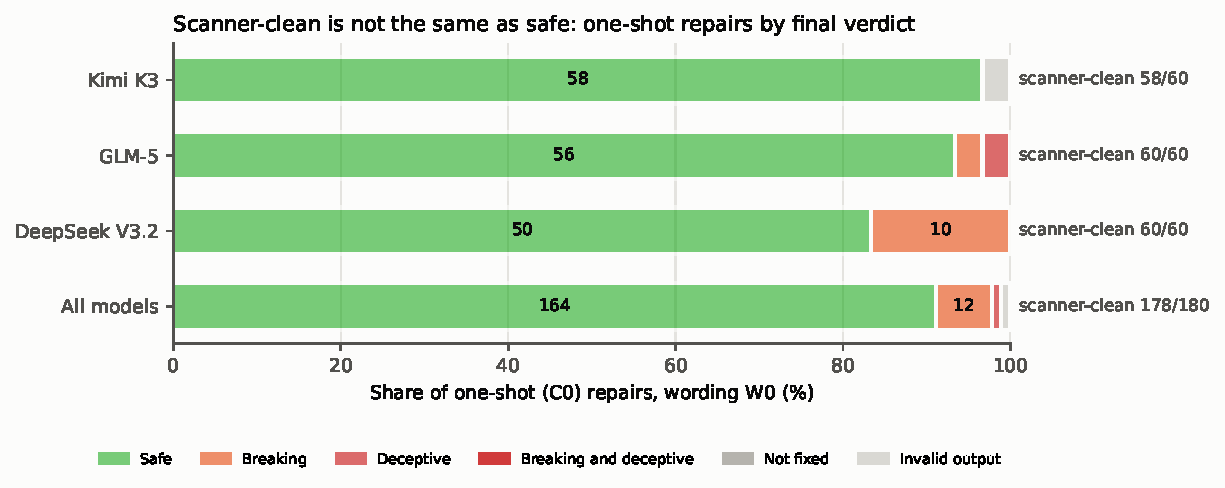
\includegraphics[width=\linewidth]{fig1_scanner_clean_vs_safe.pdf}
\caption{Final verdicts of one-shot (C0) repairs, wording W0.}\label{fig:c0}\end{figure}
Of the one-shot repairs, \WzeroCzeroViewScannerCleanK{} of \WzeroCzeroViewScannerCleanN{}
(\WzeroCzeroViewScannerCleanPct\%) were scanner-clean, which is what a scanner-only evaluation would report as
success. Deployed, \WzeroCzeroViewOfWhichSafeK{} of them were safe (\WzeroCzeroViewOfWhichSafePct\%,
95\% CI \WzeroCzeroViewOfWhichSafeLo--\WzeroCzeroViewOfWhichSafeHi), \WzeroCzeroViewOfWhichBreakingK{} broke the
application and \WzeroCzeroViewOfWhichDeceptiveK{} were deceptive (Figure~\ref{fig:c0}). Over all conditions,
\WzeroOverallRqoneBreakingAmongCleanPct\% of scanner-clean repairs were breaking
(CI \WzeroOverallRqoneBreakingAmongCleanLo--\WzeroOverallRqoneBreakingAmongCleanHi) and
\WzeroOverallRqtwoDeceptiveAmongCleanPct\% deceptive
(CI \WzeroOverallRqtwoDeceptiveAmongCleanLo--\WzeroOverallRqtwoDeceptiveAmongCleanHi).

\subsection{RQ3: NetworkPolicy and model differences}
\begin{figure}[t]\centering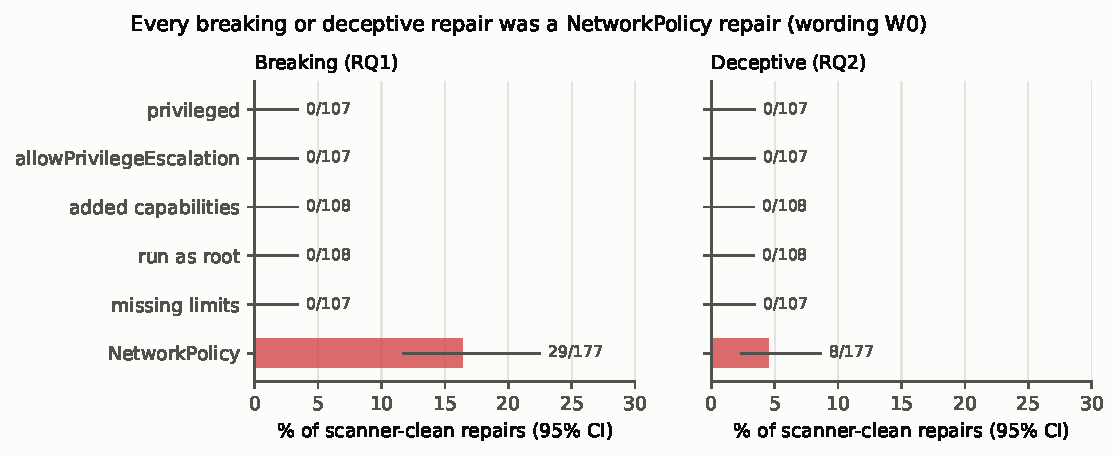
\includegraphics[width=\linewidth]{fig3_breaking_deceptive_by_type.pdf}
\caption{Breaking and deceptive repairs among scanner-clean repairs, by misconfiguration type (W0).}\label{fig:type}\end{figure}
Every breaking and every deceptive repair concerned a NetworkPolicy (Figure~\ref{fig:type}): breaking
\WzeroNetpolRqoneBreakingAmongCleanK/\WzeroNetpolRqoneBreakingAmongCleanN{}, deceptive
\WzeroNetpolRqtwoDeceptiveAmongCleanK/\WzeroNetpolRqtwoDeceptiveAmongCleanN{}; the other five types had none
(type differences: breaking $p=\WzeroRqthreeBreakingByTypeP$, deceptive $p=\WzeroRqthreeDeceptiveByTypeP$).
Breaking repairs typically restricted egress without allowing DNS or a needed dependency; deceptive repairs deleted the
namespace-wide default-deny policy. The pre-registered hypothesis that fix classes (b)+(c) break more often than (a) is
supported ($p=\WzeroHfcP$), but only through class (c): class (b) produced no breaking repair. Models differed
(breaking $p=\WzeroRqthreeBreakingByModelP$): DeepSeek~V3.2 broke \WzeroDeepseekVthreetwoRqoneBreakingAmongCleanPct\%
of its scanner-clean repairs, GLM-5 \WzeroGlmfiveRqoneBreakingAmongCleanPct\% and Kimi~K3
\WzeroKimiKthreeRqoneBreakingAmongCleanPct\%.

\subsection{RQ4: runtime feedback}
\begin{figure}[t]\centering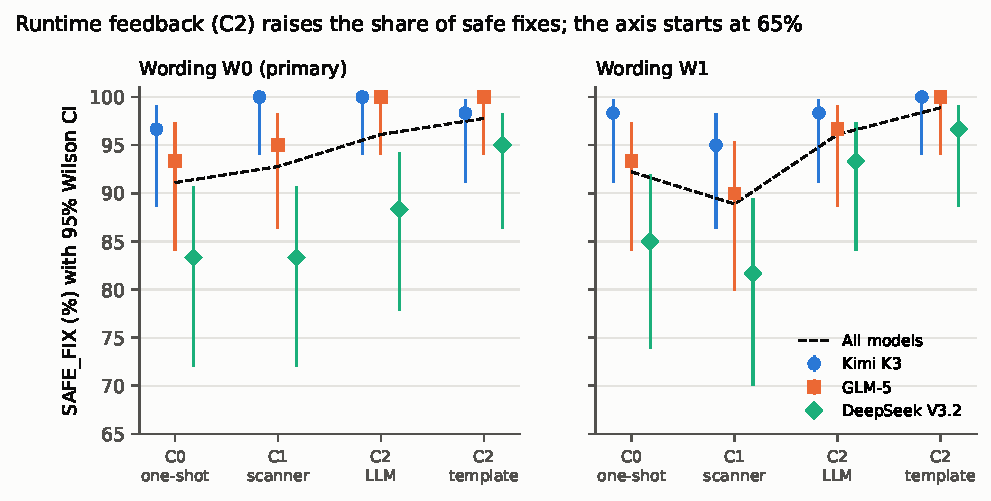
\includegraphics[width=\linewidth]{fig2_safe_by_condition.pdf}
\caption{Share of safe fixes by condition and model, both wordings.}\label{fig:cond}\end{figure}
\begin{figure}[t]\centering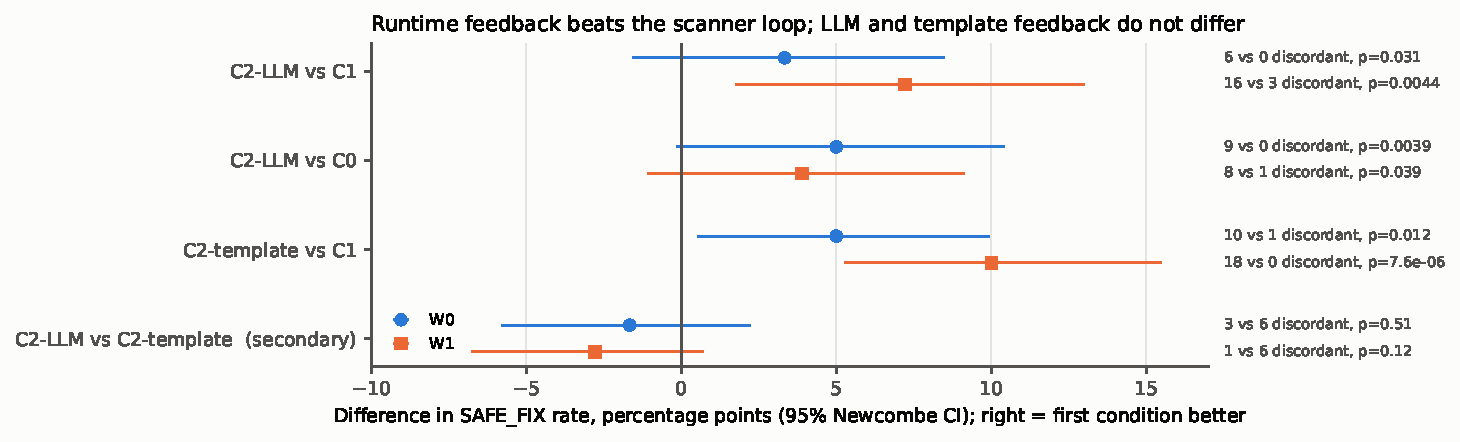
\includegraphics[width=\linewidth]{fig4_rq4_effects.pdf}
\caption{Paired comparisons of safe-fix rates (risk difference, Newcombe 95\% CI).}\label{fig:rq4}\end{figure}
Safe fixes rose from \WzeroCzeroSafePct\% (C0) and \WzeroConeSafePct\% (C1) to \WzeroCtwoLLMSafePct\% (C2-LLM)
and \WzeroCtwoTemplateSafePct\% (C2-template) (Figure~\ref{fig:cond}). All three pre-registered comparisons hold after
Holm correction: C2-LLM vs C1 ($p_\text{Holm}=\WzeroCtwoLLMVsConePholm$), C2-LLM vs C0
($p_\text{Holm}=\WzeroCtwoLLMVsCzeroPholm$), C2-template vs C1 ($p_\text{Holm}=\WzeroCtwoTemplateVsConePholm$).
The effects are a few percentage points (Figure~\ref{fig:rq4}); the unpaired Newcombe interval, as pre-registered,
includes zero for two of them while the paired test rejects. LLM-written and template feedback did not differ
($p=\WzeroCtwoLLMVsCtwoTemplateP$): the benefit comes from the evidence, not from a second model. The scanner-only loop
hardly improved on one shot because it stops as soon as the scanner is satisfied. Runtime feedback cost
\WzeroEffortCtwoLLMIterations{} attempts per chain on average (C1: \WzeroEffortConeIterations) and
\WzeroEffortCtwoLLMTokensPerSafe{} tokens per safe fix (C1: \WzeroEffortConeTokensPerSafe). Wording W1 showed the same
pattern.

\subsection{Robustness}
The mixed-effects regression agrees (all chains, reference C1): C2-LLM odds ratio \RegAllChainsConditionCtwoLLMOr{}
(\RegAllChainsConditionCtwoLLMOrLo--\RegAllChainsConditionCtwoLLMOrHi), C2-template
\RegAllChainsConditionCtwoTemplateOr{} (\RegAllChainsConditionCtwoTemplateOrLo--\RegAllChainsConditionCtwoTemplateOrHi),
C0 \RegAllChainsConditionCzeroOr{} (\RegAllChainsConditionCzeroOrLo--\RegAllChainsConditionCzeroOrHi).
A stratified audit of 30 chains, checked independently of the gates, agreed with every verdict.
Replaying \PeightAgreeN{} final repairs unchanged on Amazon EKS (VPC CNI network-policy enforcement) reproduced
\PeightAgreeK{} verdicts (\PeightAgreePct\%, CI \PeightAgreeLo--\PeightAgreeHi; $\kappa=\PeightKappa$), including all
\PeightNetworkPolicyK{} NetworkPolicy repairs; the one disagreement was a borderline load-test result.

\section{Threats to validity}
\paragraph{Construct validity.} \emph{Working} and \emph{secure} are what our gates measure. L5 covers four user
journeys of one application and L6 compares error rate and latency with a band measured on gold, so a repair could
break a path we do not exercise. L7 operationalises the security intent of each type with a static policy and one
runtime probe defined before any repair was run; a different probe could judge some repairs differently. The
no-regression part of L7 counts any weakened control as a failure, which is strict by design. A stratified audit of 30
chains, re-checked from the raw artifacts by a separate script independent of the gates, agreed with every verdict.

\paragraph{Internal validity.} The instrument changed twice before the protocol was frozen, both times on pilot findings
and both logged: C2 evidence and grounding fixes after the loop check, and adding no-regression results to the C2
evidence after the pilot showed C2 loops running without evidence (a bug that biased against C2). No change was made
after freezing; the analysis plan was implemented and recorded before the P7 results were read. Model outputs are not
deterministic, so every cell was repeated (three times, five for NetworkPolicy, where repeats disagreed most in the
pilot). Kimi~K3 does not accept a temperature setting and ran at its provider default; the other repairers used 0.2
and the moderator 0.0. Workers were identical instances, each qualified on gold before taking work, because load-test
results vary between hosts. The moderator never saw the gold manifests or the injected type, and an automatic check
rejected feedback containing YAML or gold-diff lines.

\paragraph{External validity.} We study one application (Online Boutique), six misconfiguration types and 18 cases,
three open-weight models served on Amazon Bedrock, and one moderator model. Other applications, especially ones with
more inter-service dependencies, other types (for example RBAC) and other models may give different rates. Most runs
used kind; replaying \PeightAgreeN{} final repairs on Amazon EKS reproduced \PeightAgreePct\% of the verdicts, including
every NetworkPolicy repair, so the main results do not depend on kind's network plugin.

\paragraph{Conclusion validity.} The RQ4 effects are a few percentage points. They hold in the pre-registered paired
tests after Holm correction and in the mixed-effects sensitivity analysis, but the unpaired Newcombe intervals include
zero for two of the three comparisons. All breaking and deceptive repairs come from one type (NetworkPolicy), so the
pooled rates mainly describe that type.

\paragraph{Literature review.} One researcher screened all records; a blind second screener re-screened a 20\% sample
at both stages (title/abstract: 94.7\% agreement, $\kappa=0.85$; full text: 89.2\%, $\kappa=0.75$, before resolution).
Two full-text disagreements were resolved in favour of the second screener, which removed two studies from the included
set. The second screener was an independent AI session given only the criteria and the sampled records, which is weaker
than a second human and is reported as such. \LitNotRetrieved{} full texts (mostly book chapters) could not be obtained; they are listed by name. Semantic Scholar and OpenAlex do not index every included study, so
snowballing could not follow all reference lists.

\section{Conclusion}
Judging LLM security repairs by whether a scanner stops complaining overstates their quality. On a deployed
microservice application, \WzeroCzeroViewOfWhichBreakingPct\% of the scanner-clean one-shot repairs broke the
application and \WzeroCzeroViewOfWhichDeceptivePct\% left the security intent unmet. The failures concentrate where a
fix depends on how the application's services talk to each other: every breaking and every deceptive repair concerned
a NetworkPolicy. Feeding runtime evidence back to the model raised the share of safe fixes above a scanner-only loop,
and a fixed template did as well as an LLM-written message, so what helps is the evidence, not a second model. Our
review of \LitIncluded{} studies found none that combines deployment, application checks and a runtime check of the
security intent. We recommend that evaluations of automated configuration repair deploy the result and check both that
the application still works and that the fix does what it is meant to do, at least for repairs that change how
components communicate.

\section*{Data availability}
The replication package contains the frozen protocol and every logged deviation, the gold manifests and the 18 cases
with their injectors, intent policies and probes, the harness and worker image definition, the prompts with their
hashes, all model inputs and outputs and gate evidence for every attempt, the analysis scripts that produce every number,
table and figure in this paper, and the literature-review records, screening decisions, extraction table and scripts.
% TODO (Abdul): repository URL and archive DOI (e.g. Zenodo) once the repository is made public.
Repository: \texttt{[URL to be added]}; archived copy: \texttt{[DOI to be added]}.
\bibliographystyle{plain}
\bibliography{references}
\end{document}
